% !TEX encoding = UTF-8
% !TEX TS-program = pdflatex
% !TEX root = ../tesi.tex

%**************************************************************
\chapter{Background tecnologico} \label{background}
%**************************************************************

Lo scopo di questo capitolo è la presentazione delle tecnologie utilizzate durante lo sviluppo di moviORDER. La realizzazione dell'applicazione ha permesso l'apprendimento di nuove tecnologie e l'approfondimento di alcune già in parte conosciute. Parte delle tecnologie sono state scelte dallo stagista in seguito al completamento dell'analisi dei requisiti, mentre la maggior parte sono state imposte dal tutor aziendale o dal dominio del problema. Le tecnologie scelte dallo stagista sono state concordate con il team di sviluppo di \visione{}. Le prossime sezioni presentano le tecnologie in base al contesto in cui sono state utilizzate.

\section{Framework}	

La presentazione delle tecnologie utilizzate per lo sviluppo di moviORDER inizia dalla scelta del framework, in quanto la scelta del framework ha imposto l'utilizzo di parte dei linguaggi di programmazione usati durante il periodo di stage. Per lo sviluppo del progetto è stato proposto l'utilizzo di un framework cross-platform in quanto è stata richiesta la realizzazione di un'applicazione che funzionasse in ambiente Android e iOS. Data la diversità delle tecnologie richieste per lo sviluppo di codice nativo Android e iOS, e la limitata quantità di tempo a disposizione per la realizzazione del progetto, l'utilizzo di un framework cross-platform era la migliore soluzione per portare a termine il progetto nei tempi richiesti. Allo stagista era permesso di scegliere tra due \glossaryItem{framework cross-platform}: Xamarin e PhoneGap.\\ Vengono di seguito descritti:
\begin{enumerate}
	\item le motivazioni alla base dei framework cross-platform;
	\item gli approcci alla base dei framework cross-platform;
	\item il framework Xamarin;
	\item il framework PhoneGap;
	\item le motivazioni che hanno portato PhoneGap a prevalere su Xamarin.
\end{enumerate}

\subsection{Motivazioni alla base dei framework cross-platform}

Al giorno d'oggi è inpensabile realizzare un'applicazione mobile per una sola piattaforma perché il mercato è eccessivamente frammentato. Quindi se si dovesse scegliere di sviluppare un'applicazione per una sola piattaforma si perderebbe una potenziale parte di mercato e quindi di clienti. La seguente figura mostra, a scopi illustrativi, la frammentazione del mercato italiano nel 2016.

\begin{figure}[!h] 
    \centering 
    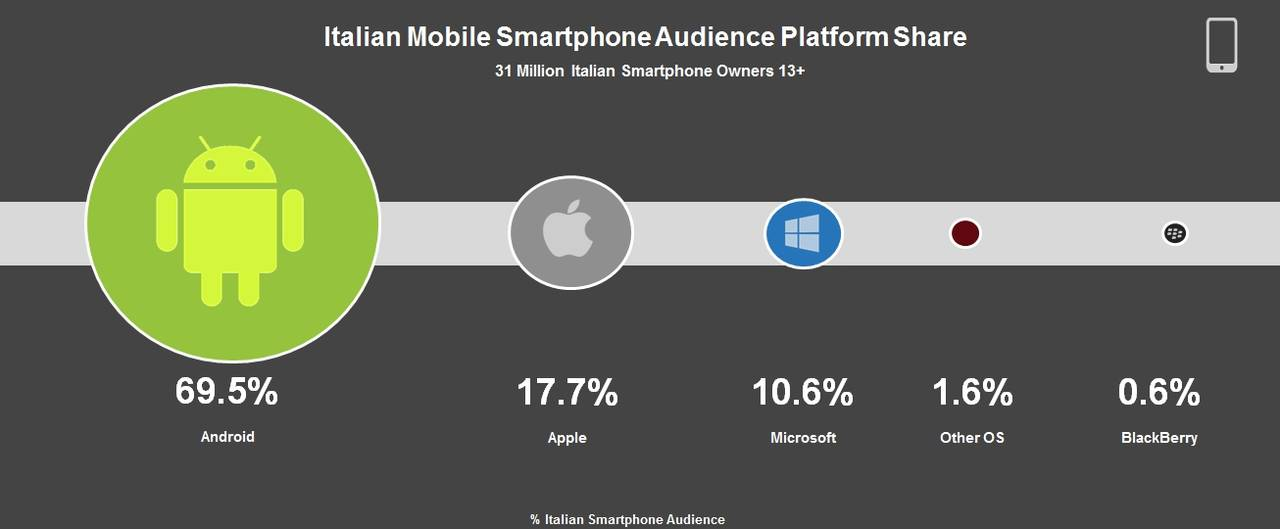
\includegraphics[width=\columnwidth]{tecnologie/mercato} 
    \caption{Frammentazione SO del mercato italiano nel 2016}
\end{figure}

Compresa la necessità di sviluppare più versioni della medesima applicazione in diverse piattaforme, il problema si sposta sulle risorse economiche e sul tempo che si ha a disposizione per lo sviluppo. Infatti lo sviluppo in differenti piattaforme comporta l'utilizzo di differenti linguaggi di programmazione e quindi la necessità di più programmatori esperti, precisamente almeno uno per piattaforma. Altre variabili di cui tener conto sono gli strumenti di sviluppo necessari, le API che si hanno a disposizione e fattori quali i sensori disponibili sui dispositivi, la dimensione degli schermi e le capacità di calcolo differenti.

L'obiettivo che i framework cross-platform cercano di raggiungere è la risoluzione di tutti questi problemi in maniera efficiente ed efficace in termini di risorse utilizzate, quindi, più precisamente, di ridurre gli effetti negativi della frammentazione del mercato.

\begin{figure}[!h] 
    \centering 
    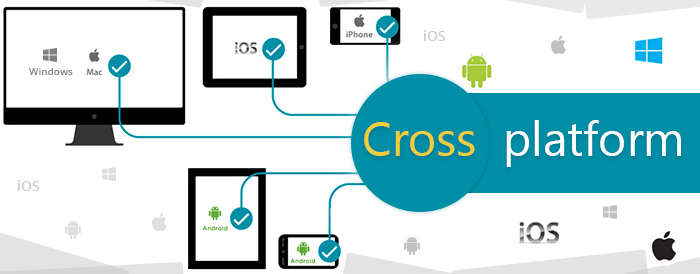
\includegraphics[width=\columnwidth]{tecnologie/framework} 
    \caption{L'obiettivo dei framework cross-platform}
\end{figure}

Per raggiungere questo obiettivo i framework cross-platform permettono l'utilizzo di un solo linguaggio di programmazione, o di un insieme ristretto di linguaggi, per lo sviluppo di un unico codice sorgente che viene poi in secondo luogo convertito nel codice nativo delle piattaforme sulle quali si desidera distribuire l'applicazione. 

Per concludere, dati oggettivi dimostrano che durante il 2016 l'utilizzo dei framework cross-platform ha portato ad un risparmio in termini di risorse economiche nell'80\% dei casi e ad un risparmio di tempo nell'83\% dei casi.

\subsection{Approcci alla base dei framework cross-platform}

Per la scelta del framework cross-platform più idoneo al problema è stato richiesto di studiare gli approcci secondo i quali i framework permettono la distribuzione su varie piattaforme. Esistono principalmente quattro approcci in base ai quali i framework possono essere classificati:
\begin{itemize}
	\item approccio web;
	\item approccio ibrido;
	\item approccio interpretato;
	\item approccio cross-compiled.
\end{itemize}

In questa tesi vengono presentati solamente l'approccio ibrido e quello interpretato, poiché utilizzati dai framework proposti dal tutor aziendale.

L'approccio ibrido si interpone tra la realizzazione di un'applicazione web e lo sviluppo di un'applicazione mobile in codice nativo. In questo tipo di approccio l'applicazione viene sviluppata utilizzando tecnologie web ed eseguita all'interno di un container nativo sul dispositivo mobile. Per eseguire l'applicazione viene utilizzato il motore di rendering del browser del dispositivo mobile che si occupa di interpretare e visualizzare il contenuto HTML dell'applicazione tramite una visualizzazione web a schermo intero. L'accesso alle funzionalità native offerte dal dispositivo mobile è permesso grazie ad un livello astratto che si interpone tra l'applicazione ibrida e tali funzionalità. Questo livello astratto espone le funzionalità tramite API Javascript. 

\begin{figure}[!h] 
    \centering 
    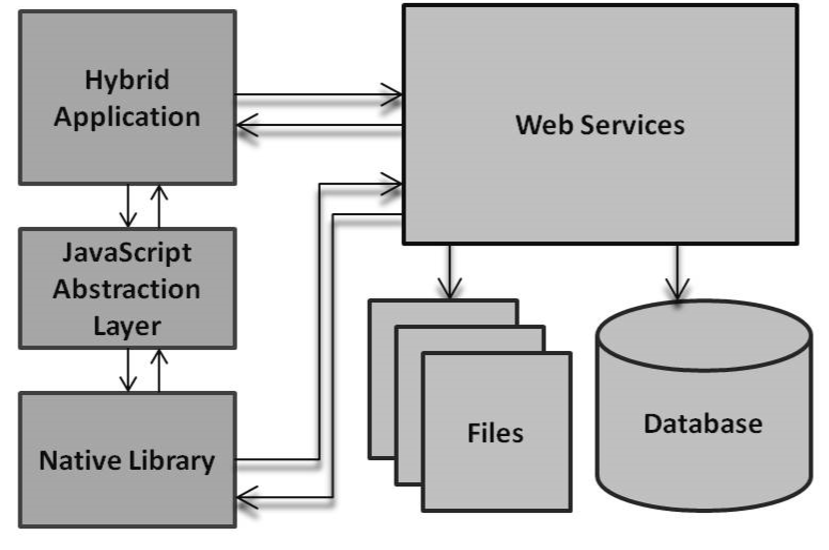
\includegraphics[width=0.9\columnwidth]{tecnologie/ibrido} 
    \caption{Architettura di un'applicazione ibrida}
\end{figure}

Nel caso delle applicazioni interpretate il codice sorgente dell'applicazione viene distribuito sul dispositivo mobile e in seguito interpretato da un interprete che si occupa di eseguire il codice a run-time. Anche in questo caso le funzionalità native vengono rese disponibili da un livello astratto. La caratteristica principale dell'interprete è che eseguendo il codice sorgente su differenti piattaforme, esso supporta lo sviluppo cross-platform delle applicazioni. L'applicazione interpretata interagisce con il livello astratto per accedere alle API native. Uno dei vantaggi dell'approccio interpretato è che utilizza elementi delle specifiche interfacce utente native per l'interazione utente. Infine, la logica applicativa è catturata in maniera del tutto indipendente dalla piattaforma sulla quale l'applicazione viene eseguita.

\begin{figure}[!h] 
    \centering 
    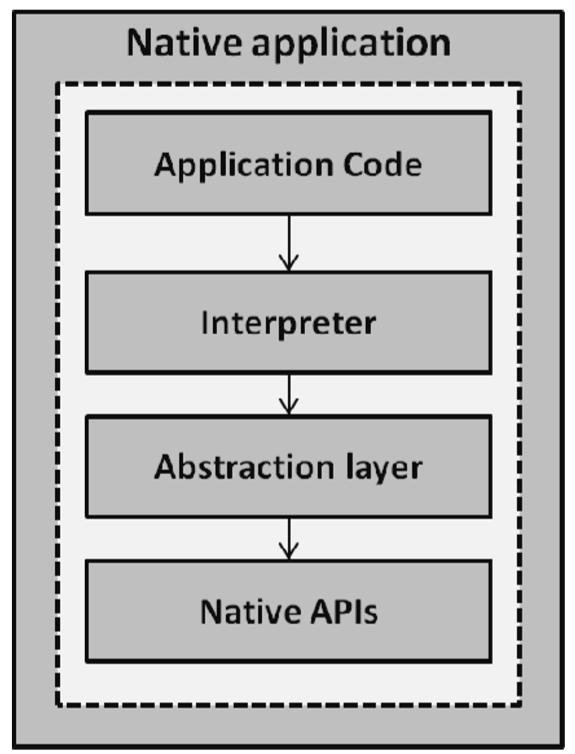
\includegraphics[height=8cm,width=0.6\columnwidth]{tecnologie/interpretato} 
    \caption{Architettura di un'applicazione interpretata}
\end{figure}

\newpage

\subsection{Xamarin}

Si tratta di un framework cross-platform di proprietà dell'azienda Microsoft che utilizza due approcci differenti, l'approccio interpretato per l'ambiente Android e Windows, e l'approccio compilato per l'ambiente iOS. Più precisamente, per le piattaforme Android e Windows è possibile generare l'applicazione direttamente tramite i tool messi a disposizione dal framework e successivamente distribuirla sui rispettivi store, mentre per la piattaforma iOS è necessario un passo aggiuntivo. È richiesto, infatti, il passaggio per una macchina Apple che abbia installato XCode per eseguire la compilazione dell'applicazione. Infine, Xamarin richiede che venga utilizzato il linguaggio C\# per lo sviluppo dell'applicazione. Nella figura sottostante viene presentata l'architettura di Xamarin.

\begin{figure}[!h] 
    \centering 
    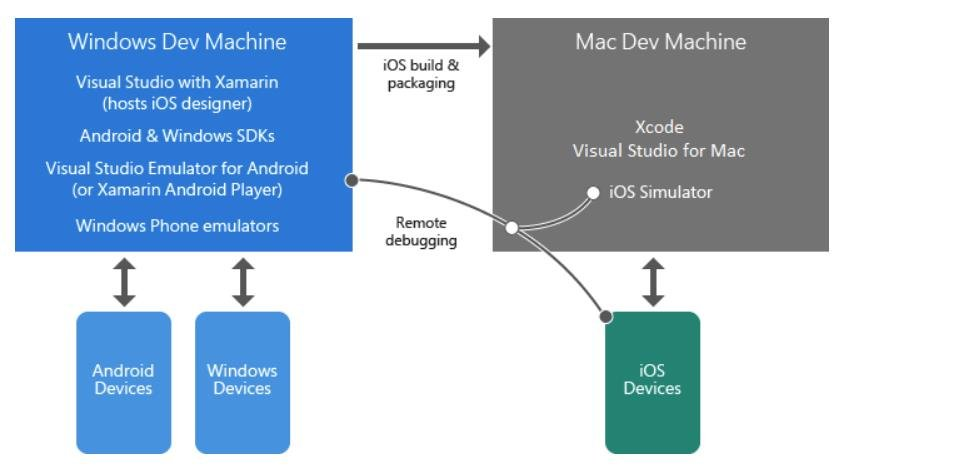
\includegraphics[width=\columnwidth]{tecnologie/xamarinArchitecture} 
    \caption{Architettura del framework Xamarin}
\end{figure}

\subsection{PhoneGap}

Si tratta di un framework cross-platform di proprietà dell'azienda Apache che utilizza un approccio di tipo ibrido. Quindi permette la realizzazione di applicazioni mobile tramite l'utilizzo di tecnologie web, che sono al giorno d'oggi strumenti conosciuti da tutti gli sviluppatori. L'accesso ai componenti hardware dei dispositivi mobile è permesso grazie all'utilizzo di plugin scaricabili dalla pagina ufficiale del framework. Vantaggi importanti del framework sono la presenza di documentazione completa per i plugin e la presenza di una community grande e sempre disponibile. Infine PhoneGap rende disponibili degli strumenti che facilitano lo sviluppo dell'applicazione: PhoneGap Desktop App, PhoneGap CLI, PhoneGap App e PhoneGap Build. I primi tre strumenti fanno parte dell'ambiente di sviluppo utilizzato durante lo stage e verranno descritti successivamente. PhoneGap Build è uno strumento che permette la build dell'applicazione direttamente su un server cloud Adobe a partire da un file zip contenente la cartella con il codice sorgente dell'applicazione. In seguito alla build è possibile generare e scaricare automaticamente l'applicazione per Windows o per Android. Per quanto riguarda iOS, è necessario fornire i certificati richiesti da Apple per la distribuzione dell'applicazione. Nella pagina successiva vengono presentate l'architettura di PhoneGap e una figura illustrativa di PhoneGap Build.

\begin{figure}[!h] 
    \centering 
    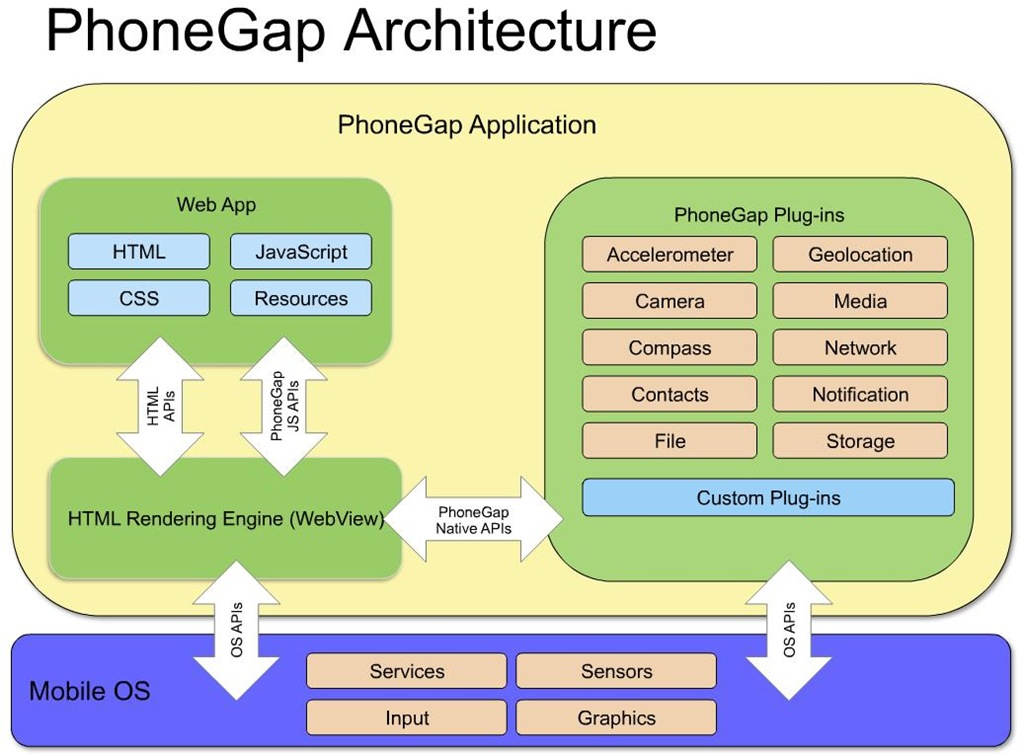
\includegraphics[width=0.9\columnwidth]{tecnologie/phonegapArchitecture} 
    \caption{Architettura del framework PhoneGap}
\end{figure}

\begin{figure}[!h] 
    \centering 
    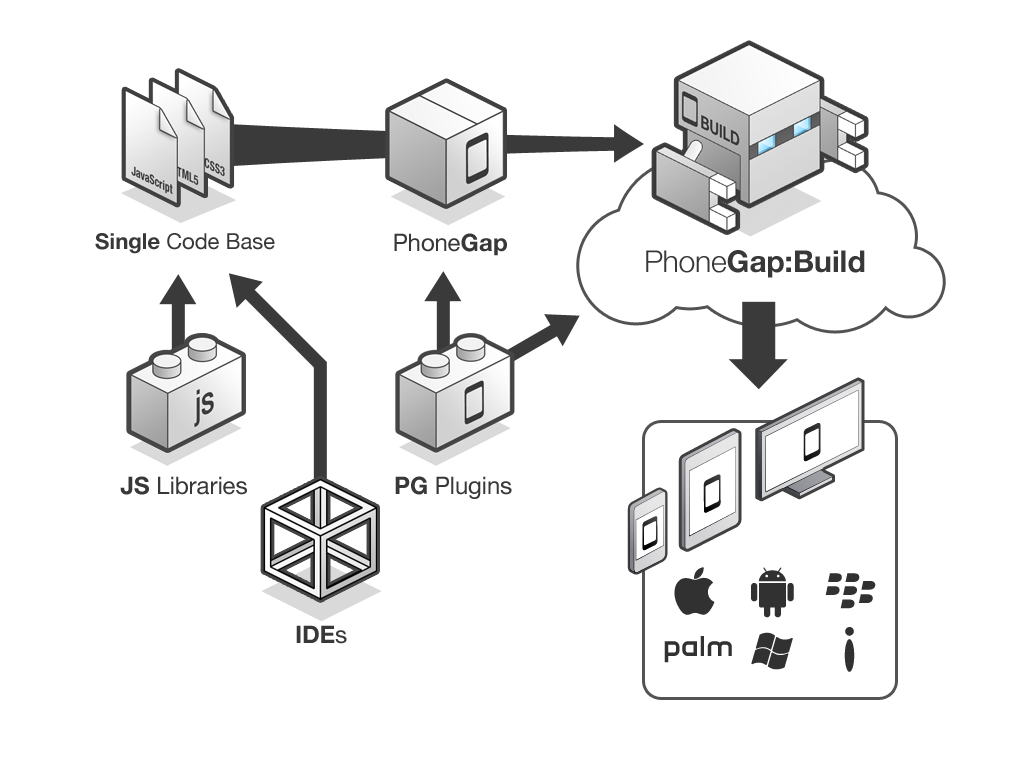
\includegraphics[width=\columnwidth]{tecnologie/phonegapBuild} 
    \caption{Figura illustrativa di PhoneGap Build}
\end{figure}

\newpage


\subsection{La scelta di PhoneGap}

Lo stagista ha optato per il framework PhoneGap per tre motivi sostanziali:
\begin{enumerate}
	\item \textbf{linguaggio di programmazione}: PhoneGap richiedeva l'utilizzo di tecnologie web, già conosciute e apprese dallo stagista all'Università. Lo studio del linguaggio C\#, utilizzato da Xamarin, avrebbe richiesto un periodo di formazione che avrebbe sforato le 40 ore messe a disposizione per la formazione sulle tecnologie;
	\item \textbf{linguaggio Javascript}: come detto precedentemente, lo stagista era interessato ad approfondire il linguaggio Javascript, richiesto al giorno d'oggi dalla maggior parte delle aziende che si occupano della realizzazione di applicazioni web;
	\item \textbf{facilità nello sviluppo dell'interfaccia grafica}: utilizzando tecnologie web risultava semplice progettare e sviluppare un'interfaccia grafica \glossaryItem{responsive}, e quindi in grado di adattarsi alla maggior parte dei dispositivi mobile presenti sul mercato.
\end{enumerate}

\section{Ambiente di sviluppo}

Durante il periodo di stage è stato utilizzato uno specifico ambiente di lavoro, comprendente tecnologie in parte imposte dal tutor aziendale e in parte scelte dallo stagista. La qualità di queste tecnologie ha impatto diretto sulla qualità di processo e quindi sulla qualità di prodotto, per cui è importante tenere l'ambiente di lavoro costantemente completo, ordinato e aggiornato. Per ottenere questo, lo stagista ha dovuto analizzare le tecnologie scelte per assicurarsi che fossero le più adatte per il dominio del problema.

\subsection{Suite di PhoneGap}

La suite di PhoneGap ha costituito parte fondamentale dell'ambiente di lavoro. Sono stati utilizzati i seguenti software della suite:
\begin{itemize}
	\item \textbf{PhoneGap Desktop App}: utilizzata inizialmente per prendere dimestichezza con il framework;
	\item \textbf{PhoneGap CLI}: utilizzata dopo aver preso dimestichezza con il framework;
	\item \textbf{PhoneGap App}: utilizzata inizialmente per testare l'applicazione generata dal framework.
\end{itemize}

PhoneGap Desktop App è un'applicazione installabile su Windows o Mac con la quale è possibile iniziare ad utilizzare il framework con estrema facilità. Essa fornisce un'interfaccia grafica per la creazione, la gestione e il testing di progetti PhoneGap. Per testare l'applicazione è sufficiente essere in possesso di un dispositivo Android con installata l'applicazione PhoneGap App. L'applicazione in versione iOS è stata rimossa dall'App Store per non aver passato i controlli di qualità Apple. Nella pagina successiva viene presentata una figura che mostra l'interfaccia grafica di PhoneGap Desktop App.

\begin{figure}[!h] 
    \centering 
    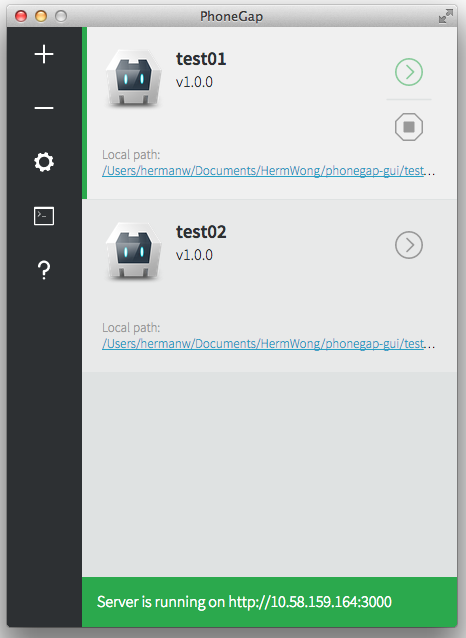
\includegraphics[width=0.8\columnwidth]{tecnologie/phonegapDesktop} 
    \caption{PhoneGap Desktop App}
\end{figure}

\newpage

PhoneGap CLI estende le funzionalità offerte da PhoneGap Desktop App tramite un'interfaccia a riga di comando. Tale applicazione era lo strumento principale per l'utilizzo di PhoneGap prima della creazione dell'app desktop. PhoneGap CLI può essere utilizzata singolarmente o assieme a PhoneGap Desktop App e/o PhoneGap Build.

PhoneGap App è un'applicazione mobile, installabile solamente su dispositivi Android, con la quale è possibile testare l'applicazione PhoneGap senza generare ed installare nessun file applicazione. Per testare l'applicazione è sufficiente avviare l'esecuzione del progetto su PhoneGap Desktop App e collegare il computer di sviluppo e il dispositivo su cui è installata PhoneGap App alla stessa rete Wi-Fi. Dopo aver completato questi semplici passaggi, viene richiesto di inserire su PhoneGap App l'indirizzo di rete su cui il progetto è stato messo in esecuzione da PhoneGap Desktop App. Dopo aver inserito questo indirizzo, la reale applicazione verrà visualizzata sullo smartphone e sarà possibile testarla completamente.

\begin{figure}[!h] 
    \centering 
    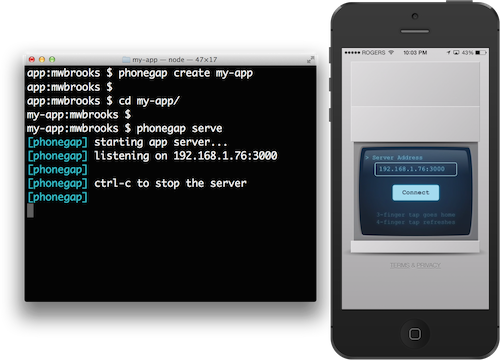
\includegraphics[width=0.8\columnwidth]{tecnologie/phonegapCLIApp} 
    \caption{PhoneGap CLI e PhoneGap App}
\end{figure}

\subsection{Editor e IDE}

\subsubsection{Sublime Text 3.0}

Per lo sviluppo del progetto PhoneGap è stato utilizzato l'editor Sublime Text 3.0, ritenuto dallo stagista il più semplice e leggero per la realizzazione di applicazioni web. 

\begin{figure}[!h] 
    \centering 
    
\includegraphics[height=4cm,width=4cm]{tecnologie/sublime} 
    \caption{Logo di Sublime Text 3.0}
\end{figure}

\subsubsection{Android Studio}

Durante lo stage, l'applicazione Android generata tramite i tool offerti dal framework PhoneGap non era soddisfacente: spesso non funzionava o l'interfaccia grafica non rispecchiava quella desiderata. Per cui è stato necessario installare Android Studio per applicare gli accorgimenti in codice nativo necessari a rendere l'app usabile. Android Studio è un ambiente di sviluppo integrato (IDE) basato sul software di JetBrains IntelliJ IDEA e progettato specificamente per lo sviluppo di applicazioni Android.

\begin{figure}[!h] 
    \centering 
    
\includegraphics[height=4.5cm,width=4.5cm]{tecnologie/androidStudio} 
    \caption{Logo di Android Studio}
\end{figure}

\subsubsection{XCode}

Durante lo stage, l'applicazione iOS generata tramite i tool offerti dal framework PhoneGap non era soddisfacente: spesso non funzionava o l'interfaccia grafica non rispecchiava quella desiderata. Per cui è stato necessario installare XCode per applicare gli accorgimenti in codice nativo necessari a rendere l'app usabile. Xcode è un ambiente di sviluppo integrato (IDE) contenente una suite di strumenti utili allo sviluppo di software per i sistemi macOS, iOS, watchOS e tvOS. È completamente sviluppato e mantenuto da Apple.

\begin{figure}[!h] 
    \centering 
    
\includegraphics[height=4cm,width=5cm]{tecnologie/xCode} 
    \caption{Logo di XCode}
\end{figure}

\subsubsection{Eclipse JEE}

Durante lo stage è stata richiesta la realizzazione di un servizio web che si interponesse tra la logica applicativa di moviORDER e il database presente sul server Azure di \visione{}. Il servizio web è stato realizzato in linguaggio Java tramite l'utilizzo di oggetti servlet. Per la realizzazione degli oggetti servlet è stato utilizzato l'IDE Eclipse JEE che offre buoni strumenti per lo sviluppo di applicazioni web Java. Eclipse è un ambiente di sviluppo integrato multi-linguaggio e multipiattaforma, ideato da un consorzio di grandi società quali Ericsson, HP, IBM, Intel, MontaVista Software, QNX, SAP e Serena Software, chiamato Eclipse Foundation.

\begin{figure}[!h] 
    \centering 
    
\includegraphics[width=0.8\columnwidth]{tecnologie/eclipse} 
    \caption{Logo di Eclipse}
\end{figure}

\subsection{Gestione DBMS}

Durante il progetto, per la gestione del database di moviORDER è stato utilizzato il DBMS Microsoft SQL Server. Per una gestione veloce ed ottimale dello stesso si è deciso di usare il software SQL Server Management Studio. SQL Server Management Studio (SSMS) è un'applicazione software usata per configurare, gestire e amministrare database, in locale o su un server cloud, con il DBMS Microsoft SQL Server. 

\begin{figure}[!h] 
    \centering 
    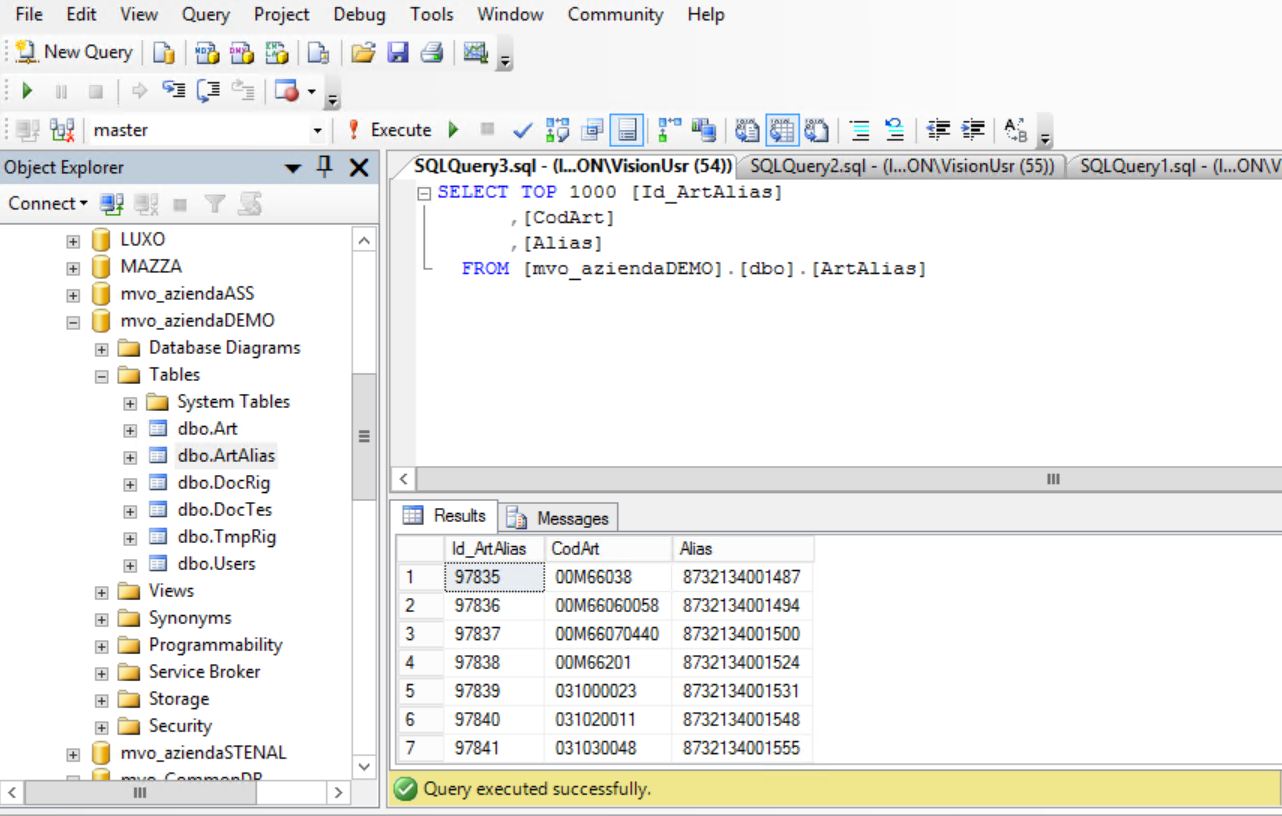
\includegraphics[width=\columnwidth]{tecnologie/ssms} 
    \caption{Screenshot di SQL Server Management Studio}
\end{figure}

\newpage

\subsection{Server web}

Per lo sviluppo del progetto è stato realizzato un servizio web che fornisce una API all'applicazione per poter accedere ai dati contenuti nel database sul server cloud di \visione{}. Per permettere l'esecuzione del servizio web sul server cloud si è utilizzato Apache Tomcat. Apache Tomcat (o semplicemente Tomcat) è un web server (nella forma di contenitore servlet) open source sviluppato dalla Apache Software Foundation. Implementa le specifiche JavaServer Pages (JSP) e servlet, fornendo quindi una piattaforma software per l'esecuzione di applicazioni Web sviluppate in linguaggio Java.

\begin{figure}[!h] 
    \centering 
    
\includegraphics[height=4cm,width=5cm]{tecnologie/tomcat} 
    \caption{Logo di Apache Tomcat}
\end{figure}

\subsection{Cloud computing}

Il servizio web e il database con il quale l'applicazione interagisce per offrire le funzionalità all'utente risiedono su un server cloud di \visione{}. Tale server è di proprietà di Microsoft Azure. Microsoft Azure (precedentemente nota come Windows Azure) è la piattaforma cloud pubblica di Microsoft, che offre servizi di cloud computing. Tramite Azure vengono erogati servizi appartenenti a diverse categorie quali: risorse di elaborazione, archiviazione e memorizzazione dati, trasmissione dati e interconnessione di reti, analisi, intelligence, apprendimento automatico, sicurezza e gestione delle identità, monitoraggio e gestione, nonché servizi per lo sviluppo di applicazioni. Per accedere al server da remoto è stato utilizzato il software Connessione Desktop Remoto di Windows.

\begin{figure}[!h] 
    \centering 
    
\includegraphics[width=0.8\columnwidth]{tecnologie/azure} 
    \caption{Logo di Microsoft Azure}
\end{figure}

\subsection{Strumenti di testing}

Durante lo sviluppo di moviORDER sono stati eseguiti dei test per verificare il corretto funzionamento del servizio web e dell'applicazione. Per il test delle API del servizio web si è utilizzato Postman. Postman è uno strumento di API testing che permette di testare API direttamente, o come parte di test d'integrazione, per determinare se soddisfano criteri di funzionalità, affidabilità, performance e sicurezza. Nel caso di moviORDER, il test avviene tramite l'invio di una richiesta HTTP POST, con parametri impostabili, alla API sul server cloud. In seguito alla richiesta il software visualizza il JSON restituito dalla API e lo sviluppatore può verificare se la risposta del servizio è quella attesa.

\begin{figure}[!h] 
    \centering 
    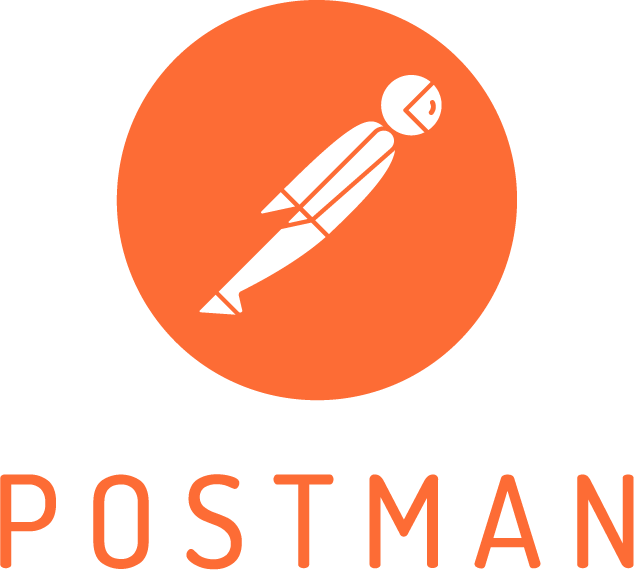
\includegraphics[height=4cm,width=5cm]{tecnologie/postman} 
    \caption{Logo di Postman}
\end{figure}

Per testare il corretto funzionamento dell'applicazione si è utilizzata la console del browser Google Chrome facente parte degli strumenti offerti dallo stesso per gli sviluppatori web. Tramite la console è stato possibile verificare la logica applicativa di moviORDER, poiché scritta in JavaScript.

\begin{figure}[!h] 
    \centering 
    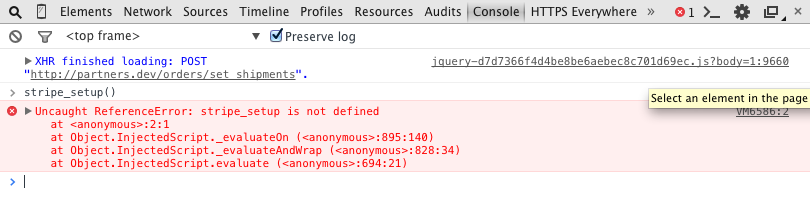
\includegraphics[width=\columnwidth]{tecnologie/console} 
    \caption{Screenshot della console di Google Chrome}
\end{figure}

\newpage

\subsection{Strumenti di versioning e ticketing}

Per scelta dello stagista il progetto è stato sottoposto a controllo di versione in ogni sua parte: applicazione, servizio web e documentazione. Questo ha permesso, principalmente nel caso dell'applicazione, di tornare a \glossaryItem{baseline} sicure nel caso di sovrascritture o perdite accidentali, o commit di codice con errori di programmazione. Per il controllo di versione si è utilizzato lo strumento Git e in particolare il servizio di hosting GitHub. Lo stagista ha scelto tali software perché già utilizzati in progetti didattici durante l'Università.

\begin{figure}[!h] 
    \centering 
    
\includegraphics[height=5cm,width=5cm]{tecnologie/git} 
    \caption{Logo di GitHub}
\end{figure}

Lo stagista ha scelto inoltre di utilizzare uno strumento di ticketing per facilitare la pianificazione del progetto. Lo strumento scelto è Asana. Asana è un'applicazione web e mobile progettata per aiutare i team ad organizzare, tracciare e gestire il loro lavoro. In particolare, lo strumento è stato utilizzato per dare una scadenza ai ticket in base alla pianificazione decisa insieme al tutor aziendale all'inizio del periodo di stage.

\begin{figure}[!h] 
    \centering 
    
\includegraphics[height=5cm,width=7cm]{tecnologie/asana} 
    \caption{Logo di Asana}
\end{figure}

\subsection{Strumenti di modellazione e documentazione}

Il progetto ha richiesto lo sviluppo di diagrammi di Gantt in fase di pianificazione e di diagrammi UML in fase di analisi dei requisiti e di progettazione. Per la costruzione dei diagrammi di Gantt è stato utilizzato il software Gantt Project, mentre per la costruzione dei diagrammi UML dei casi d'uso e delle classi è stato utilizzato il software Astah UML. I software sono stati scelti perché già appresi durante il progetto di Ingegneria del Software all'Università.

\begin{figure}[!h] 
    \centering 
    	\subfloat{
\includegraphics[width=0.3\columnwidth]{tecnologie/gantt}}
    	\subfloat{
\includegraphics[width=0.7\columnwidth]{tecnologie/astah}} 
    \caption{Logo di Gantt Project e Astah UML}
\end{figure}

Per la stesura della documentazione si è utilizzato l'editor TexMaker, anch'esso utilizzato durante il progetto di Ingegneria del Software. TexMaker permette l'inserimento veloce dei comandi \LaTeX{} più utilizzati tramite la pressione di pulsanti sull'interfaccia grafica, l'integrazione con un dizionario per il controllo ortografico e la compilazione e visione del pdf prodotto.

\begin{figure}[!h] 
    \centering 
    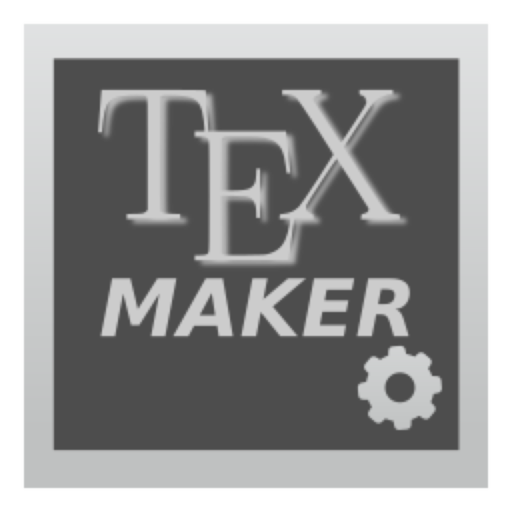
\includegraphics[height=4.5cm,width=4.5cm]{tecnologie/tex} 
    \caption{Logo di TexMaker}
\end{figure}

\subsection{Linguaggi di programmazione e murkup}

\subsubsection{HTML5, CSS3 e JavaScript}

Lo stagista ha dovuto utilizzare i linguaggi HTML5, CSS3 e JavaScript in quanto ha scelto il framework cross-platform PhoneGap, il quale richiede l'utilizzo di tecnologie web per lo sviluppo dell'applicazione mobile. In particolare, HTML5 è stato scelto perché include un insieme di funzionalità che permettono di valorizzare le interfacce mobile. Alcune di queste evidenziano come HTML5 sia già per sua natura orientato al mobile. In particolare HTML5 fornisce API per:
\begin{itemize}
	\item \textbf{geolocalizzazione}: con la scrittura di poco codice, forniscono la posizione del dispositivo in coordinate terrestri. Quindi, la stessa funzionalità su uno smartphone o un tablet fornisce la posizione dell'utente stesso;
	\item \textbf{eventi touch}: mentre i meccanismi di input nei PC consistono per lo più nella tastiera e nel mouse, nei dispositivi mobili quasi tutto passa per il touch screen, e avere funzionalità comode per gestire questo strumento consente un’interazione più ricca e senza limitazioni per l’utente. Le gestualità da attuare su un display, nel mondo mobile, costituiscono un vero e proprio linguaggio fondamentale nella user experience;
	\item \textbf{controllo batteria}: considerata l’importanza rivestita dalle risorse energetiche, l’esistenza stessa di questa libreria nel linguaggio dimostra come il suo impiego sia particolarmente mirato al panorama mobile.
\end{itemize}

Ciò che ha favorito la scelta di CSS3 sono le \glossaryItem{media queries}. Esse permettono di definire regole stilistiche in base alla tipologia del mezzo di visualizzazione, delle sue dimensioni nonchè della sua attuale disposizione (portrait o landscape). Ciò influisce non solo sull’aspetto esteriore degli elementi ma anche sul loro posizionamento e quindi sulla struttura stessa dell’interfaccia.

Per quanto riguarda il linguaggio JavaScript è stato utilizzato JavaScript puro senza l'utilizzo di framework o \glossaryItem{JQuery}. Una particolarità del linguaggio, detta AJAX, ha reso possibile eseguire chiamate alla API del servizio web di moviORDER e modificare la pagina HTML di conseguenza in base alla risposta. AJAX, acronimo di Asynchronous JavaScript and XML, è una tecnica di sviluppo software per la realizzazione di applicazioni web interattive (Rich Internet Application). Lo sviluppo di applicazioni HTML con AJAX si basa su uno scambio di dati in background fra web browser e server, che consente l'aggiornamento dinamico di una pagina web senza esplicito ricaricamento da parte dell'utente.

\begin{figure}[!h] 
    \centering 
    	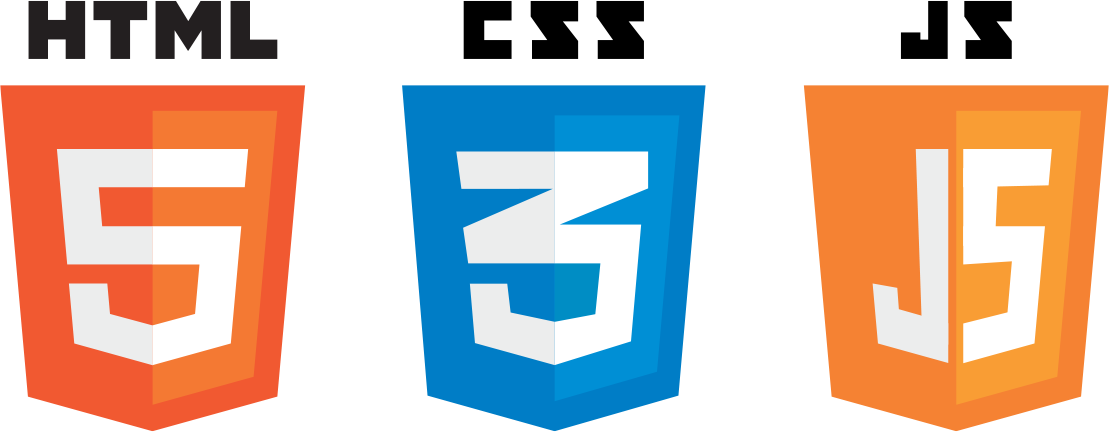
\includegraphics[width=0.8\columnwidth]{tecnologie/html5}
    \caption{Logo di HTML5, CSS3 e JavaScript}
\end{figure}

I linguaggi scelti, grazie alle loro caratteristiche che li rendono orientati al mobile, insieme ai meccanismi che il framework PhoneGap utilizza per convertire la web application in applicazione mobile, permettono di dover effettuare meno modifiche in seguito per perfezionare l'applicazione su Android e iOS.

\subsubsection{Java}

Per la realizzazione del servizio web che permette all'applicazione di interfacciarsi con il database sul server cloud di \visione{} si è utilizzato il linguaggio Java. La scelta è stata fatta dallo stagista tra due alternative in cui rientrava anche PHP. È stato scelto Java in quanto possiede un compilatore, è più facilmente debbugabile rispetto a PHP e permette l'utilizzo di oggetti servlet.  I servlet sono oggetti scritti in linguaggio Java che operano all'interno di un server web (nel caso del progetto Tomcat) oppure un server per applicazioni permettendo la creazione di applicazione web. Nel caso del progetto, i servlet hanno premesso lo sviluppo della API che costituisce il servizio web. Una descrizione della API, di come i servlet sono stati utilizzati nel progetto e di come la API viene interrogata dall'applicazione è presente in sezione §\ref{api}.

\begin{figure}[!h] 
    \centering 
    
\includegraphics[height=4.5cm,width=4.5cm]{tecnologie/java} 
    \caption{Logo di Java}
\end{figure}

\subsubsection{\LaTeX{}}

Per lo sviluppo della documentazione annessa a moviORDER è stato utilizzato il linguaggio \LaTeX{}. La scelta è ricaduta su \LaTeX{} perché già appreso e utilizzato durante il progetto di Ingegneria del Software. \LaTeX{} è un linguaggio di markup usato per la preparazione di testi basato sul programma di composizione tipografica TEX. Fornisce funzioni di desktop publishing programmabili e mezzi per l'automazione della maggior parte della composizione tipografica, inclusa la numerazione, i riferimenti incrociati, tabelle e figure, organizzazione delle pagine, bibliografie e molto altro. Infine la particolarità più utile del linguaggio è l'esistenza di community che rendono disponibili \glossaryItem{template} riutilizzabili come quello che è stato utilizzato per la stesura di questa tesi.

\begin{figure}[!h] 
    \centering 
    
\includegraphics[height=3cm,width=6cm]{tecnologie/latex} 
    \caption{Logo di \LaTeX{}}
\end{figure}

\subsection{DBMS}

Per la creazione, gestione e amministrazione di database è stato utilizzato il DBMS Microsoft SQL Server. È stato scelto questo software perché già ampiamente utilizzato all'interno dell'azienda. Questo permetterà agli sviluppatori di \visione{} di lavorare sul database di moviORDER con un linguaggio già pienamente conosciuto. Microsoft SQL Server usa una variante del linguaggio SQL standard chiamata Transact-SQL (T-SQL). Transact-SQL espande le prestazioni di SQL aggiungendo:
\begin{itemize}
	\item funzioni per controllo di flusso;
	\item possibilità di definire variabili locali;
	\item varie funzioni per la manipolazione di stringhe, date ed espressioni matematiche;
	\item miglioramento delle istruzioni DELETE e UPDATE.
\end{itemize}

\begin{figure}[!h] 
    \centering 
    
\includegraphics[height=5cm,width=7cm]{tecnologie/sqlserver} 
    \caption{Logo di SQL Server}
\end{figure}